%____________________________________________________________________________||
\section{Event selection and categorisation}
\label{sec:selection}

This section first outlines the set of ``pre-selection'' requirements
that are common to all signal and control regions, before defining the
selection criteria that are specific to each region.

%%____________________________________________________________________________||
\subsection{Common pre-selection requirements}
\label{sec:preSelection}

The event selection criteria described in this section are common to
the signal and all control regions. These selections are summarised in
Table~\ref{tab:pre-selections} and described in further detail below. 

\begin{table}[h!]
  \topcaption{Summary of the pre-selection criteria.}
  \label{tab:pre-selections}
  \centering
  \footnotesize
  \begin{tabular}{ ll }
    \hline
    \ETmiss quality               & Filters related to beam and instrumental effects, and reconstruction failures                                       \\
                                  & \parbox[t]{12cm}{
                                    Primary Vertex, 
                                    CSC Beam Halo,
                                    HBHE Noise and Isolation, 
                                    ECAL Endcap SC Noise,                                                                                               \\
                                    ECAL TP, 
                                    Bad Muon, 
                                    Bad Charged Hadron}                                                                                                 \\
    Beam halo                     & $0.1 < \mathrm{CHF} < 0.95$ for highest-\Pt jet                                                                     \\
    Jet $\mathrm{j}_i$ acceptance & Consider each jet $\mathrm{j}_i$ that satisfies $\pt^{\mathrm{j}_i} > 40\GeV$ and $\abs{\eta^{\mathrm{j_1}}} < 2.4$ \\
    Jet $\mathrm{j_1}$ acceptance & $\pt^{\mathrm{j_1}} > 100\GeV$                                                                                      \\
    Jet $\mathrm{j_2}$ acceptance & 
    $\pt^{\mathrm{j_2}} < 40\GeV$ (monojet),
    $40 < \pt^{\mathrm{j_2}} < 100\GeV$ (asymmetric),
    $\pt^{\mathrm{j_2}} > 100\GeV$ (symmetric)                                                                                                          \\
    Jets below threshold          & $\HTmiss / \ETmiss < 1.25$                                                                                          \\
    Forward jet veto              & Veto events containing a jet satisfying $\pt > 40\GeV$ and $\abs{\eta} > 2.4$                                       \\
    Energy sums                   & $\scalht > 200\GeV$ and $\HTmiss > 130\GeV$                                                                         \\
    \hline
  \end{tabular}
\end{table}

\subsubsection{MET filters}

A number of beam- and detector-related effects can induce significant
\met. Examples include beam halo, reconstruction failures, spurious
detector noise, or event misreconstruction due to detector
inefficiencies. These events, with large, non-physical values of \met,
are rejected with high efficiency by applying a range of dedicated
vetoes. All ``MET filters'' recommended by the JetMET POG and SUSY PAG
are applied by default in this analysis and listed in
Table~\ref{tab:pre-selections}.

\subsubsection{Charged hadron fraction (CHF) for leading jet}

In addition to the MET filters, a dedicated filter is applied to
remove beam halo, given that the CSC beam halo filter has been found
to be less efficient during the early Run 2 data-taking period
compared to the previous run.

Beam halo events manifest themselves as single energy deposits in the
calorimeters, which introduces large amounts of ``fake'' \met. This
effect is especially prominent in the signal region monojet category,
particularly at $\phi$ coordinates of 0 and $\pi$ because of the
tendency of halo particles to lie within the plane of the LHC ring.

Such spurious events are suppressed by requiring at least 10\% of the
for the highest-\Pt jet's energy to originate from charged
hadrons. The effectiveness of this charged hadron fraction (CHF)
requirement is demonstrated in Fig.~\ref{fig:leadJetCleaning}.

Further, a requirement of $\mathrm{CHF} < 0.95$ for the highest-\Pt
jet removes events that contain reconstruction failures concerning
muons, which are prevelant in simulated multijet events.

%There is no need for this selection in the control regions, as the
%requirement of well identified physics objects, like muons and photons
%naturally removes spurious events of this kind.

The requirement $0.1 < \mathrm{CHF} < 0.95$ for the highest-\Pt jet
can be regarded as an additional tight jet ID requirement employed by
this analysis, with efficiency close to unity for real jets and thus
not affecting the signal efficiency significantly.

\begin{figure}[h!]
    \begin{center}
        {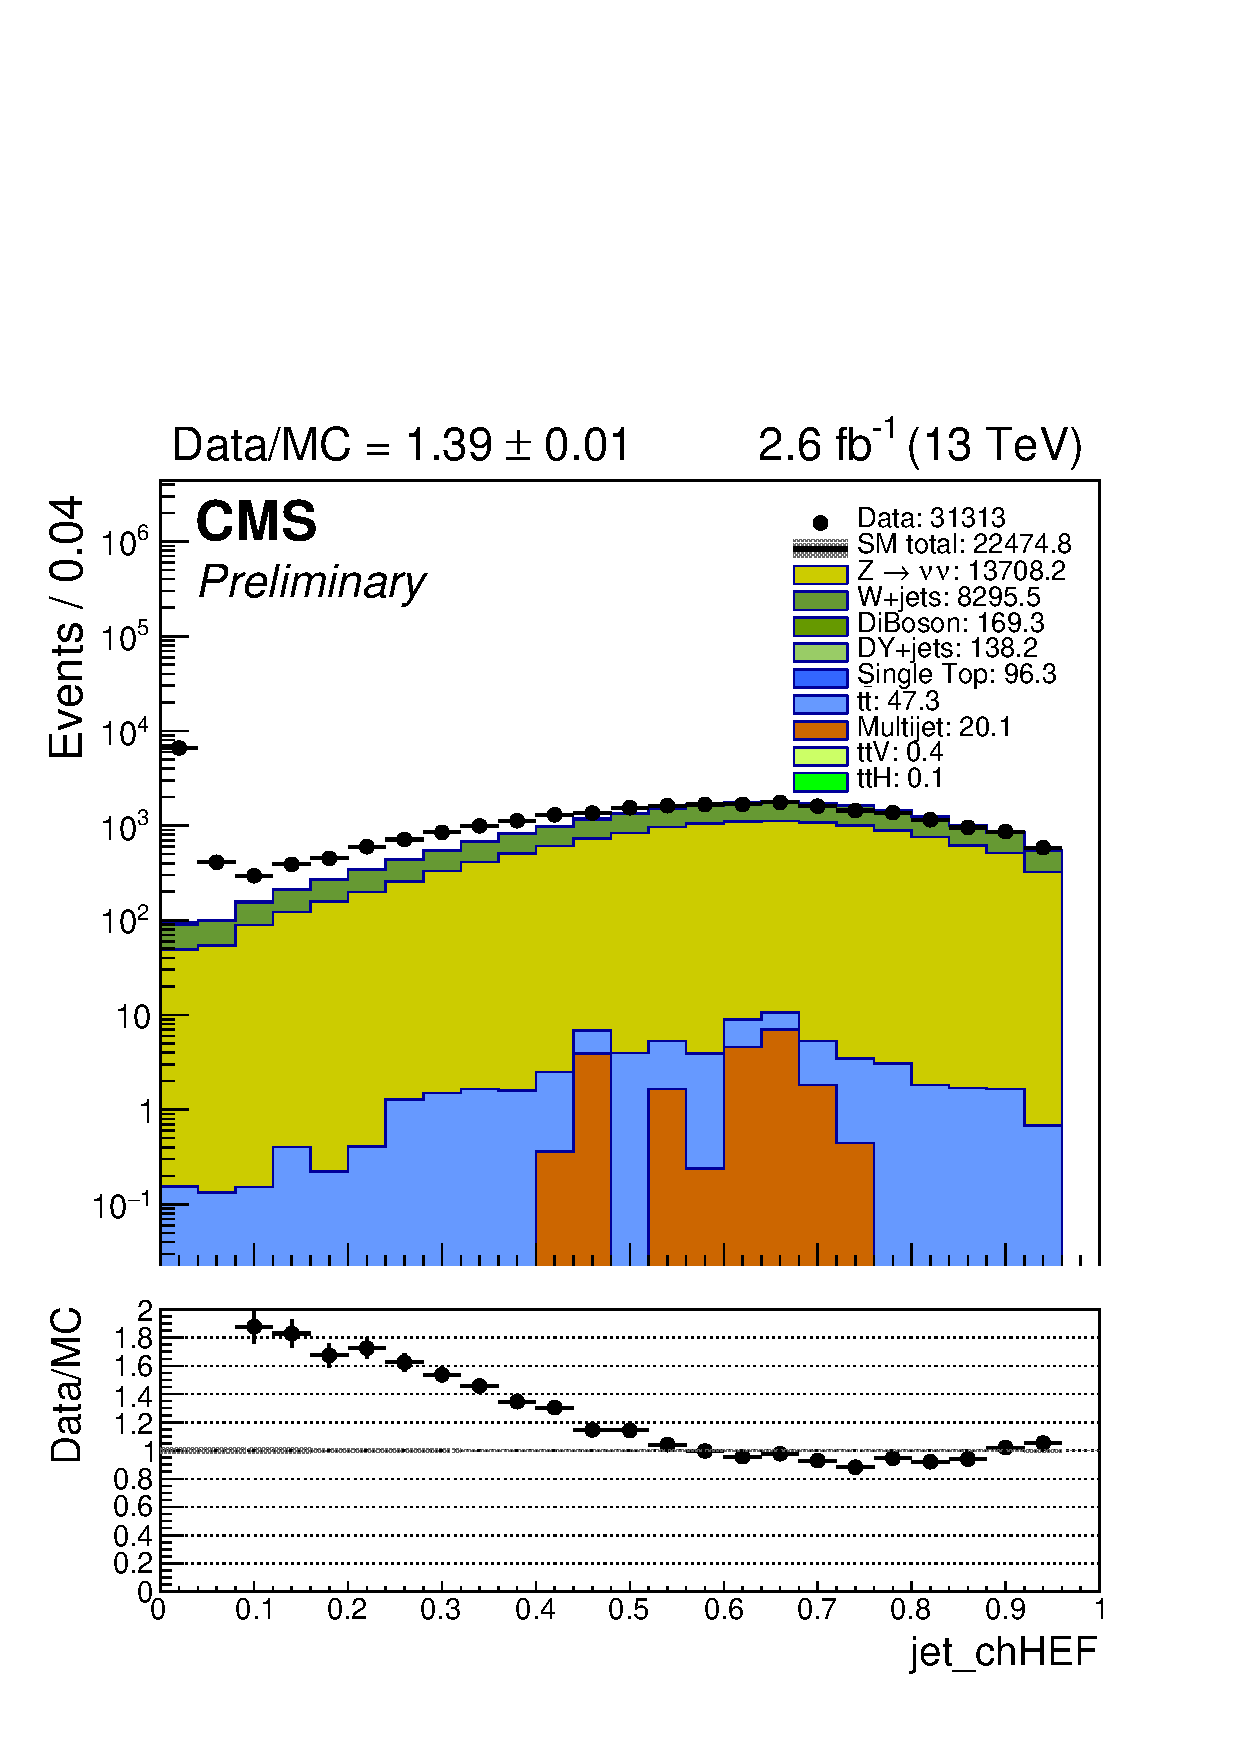
\includegraphics[width=0.32\textwidth]{figures/selection/jet_chHEF_mono_all_before.pdf}}
        {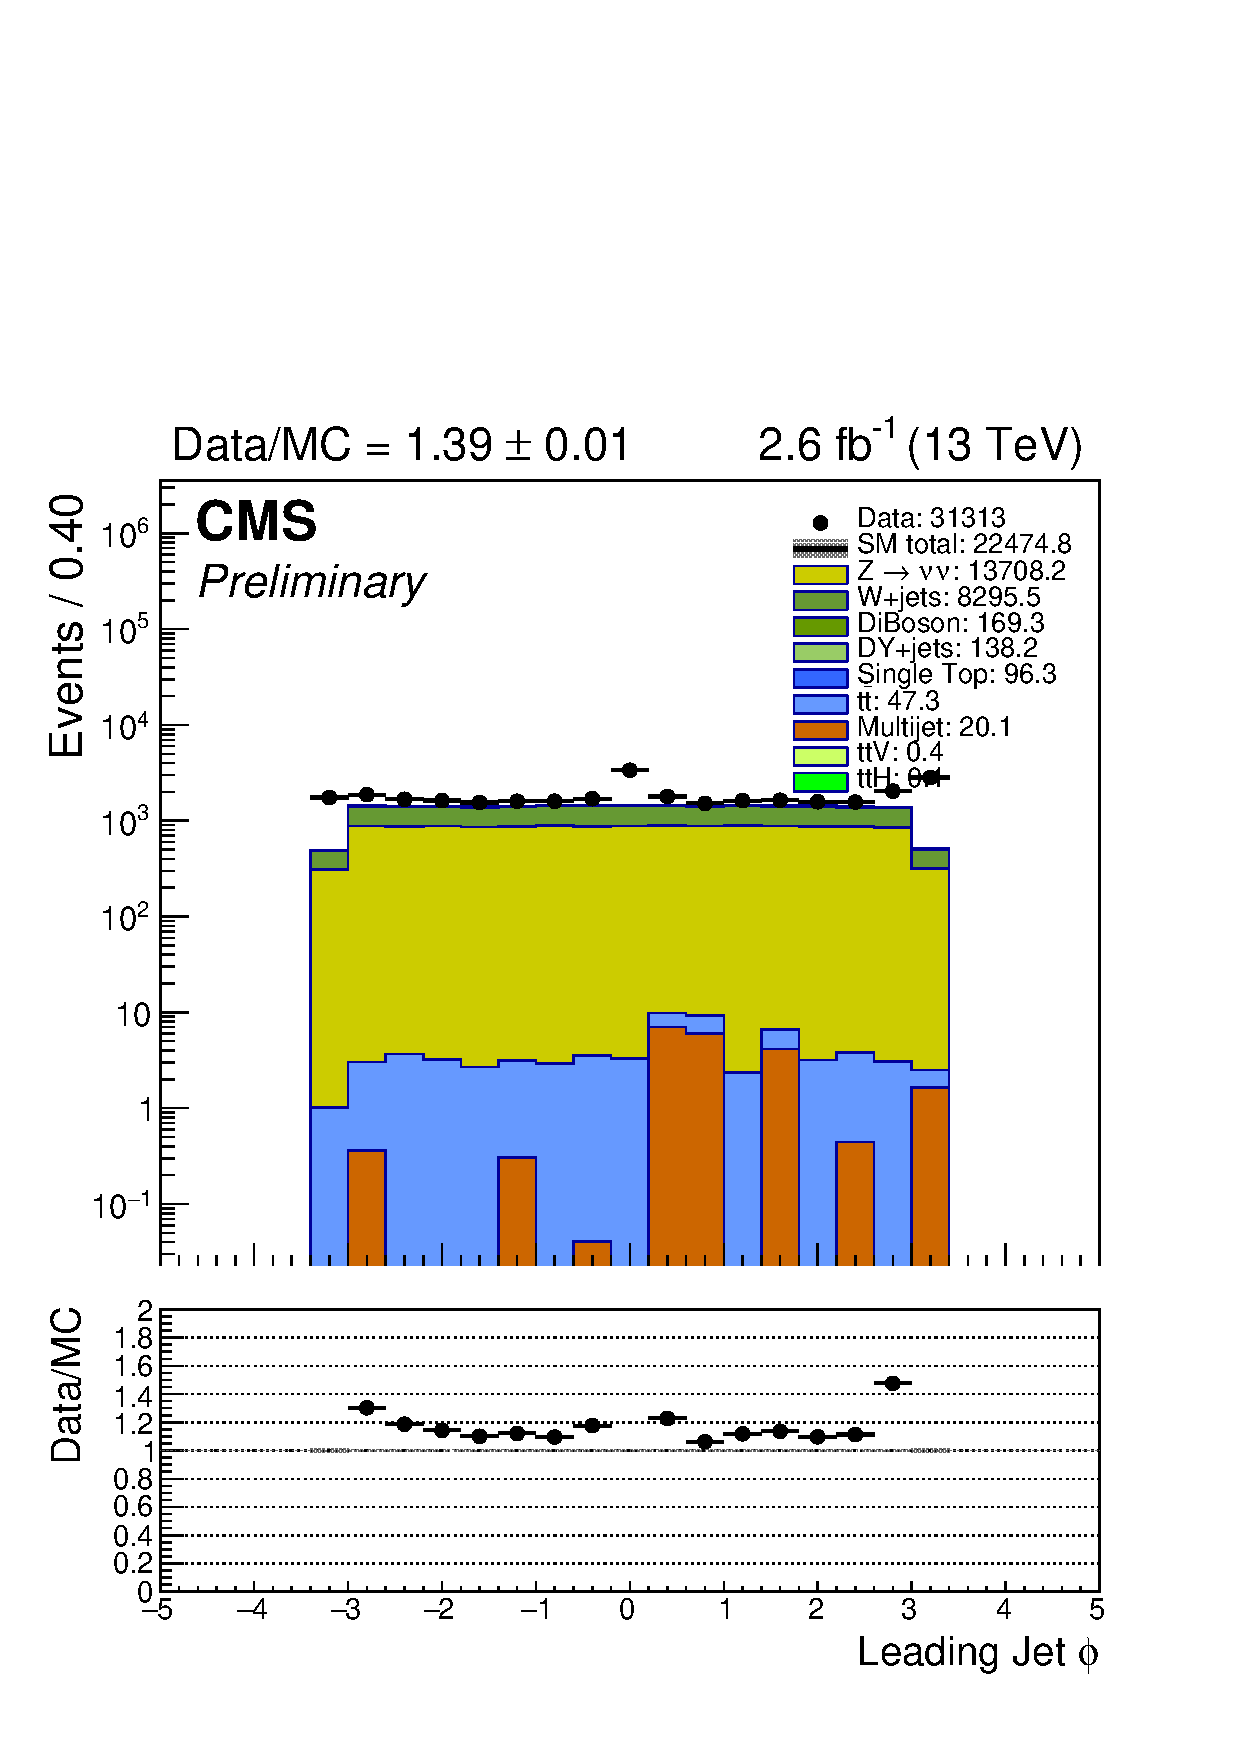
\includegraphics[width=0.32\textwidth]{figures/selection/jet_phi[0]_mono_all_before.pdf}}
        {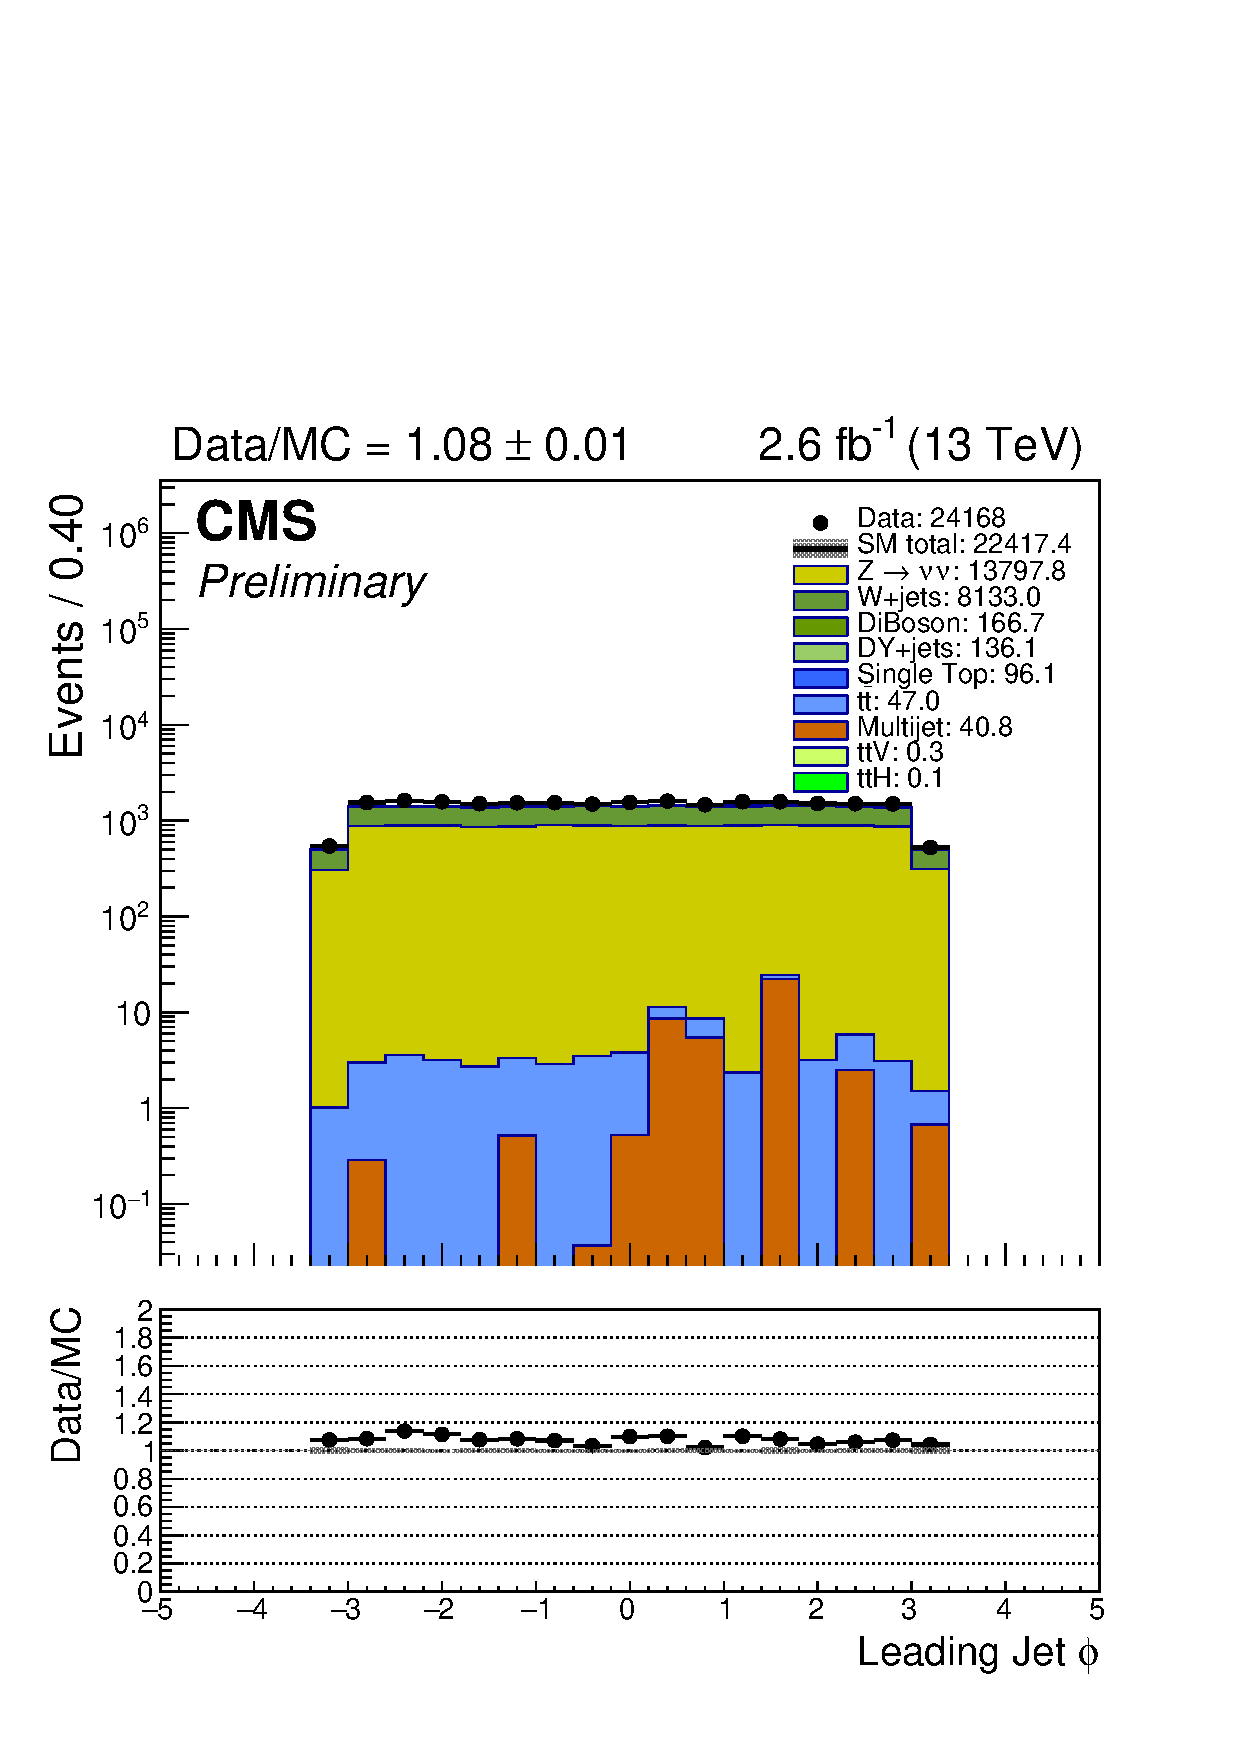
\includegraphics[width=0.32\textwidth]{figures/selection/jet_phi[0]_mono_all_after.pdf}}
        \caption{Distributions in the signal region of the jet charged
          hadron energy fraction (CHF) (Left), jet $\phi$ direction
          (Centre), and jet $\phi$ direction after applying a
          requirement of {CHF~$>0.1$}. The large excess in data at
          charged hadron fractions close to zero and ${\phi = 0, \pi}$
          is consistent with beam halo effects, and is effectively
          suppressed by the aforementioned selection.}
        \label{fig:leadJetCleaning}
    \end{center}
\end{figure}

\subsubsection{Experimental acceptance for jets}

Jets considered in the analysis are required to satisfy $\PT > 40\gev$
and $|\eta| < 2.4$. The selected jets are used in the calculation of
all jet-based event-level variables, such as \njet, \HT, \mht, and
\alphat (see Sec.~\ref{} for their definitions).

The highest-\Pt jet in the event is required to satisfy $\Pt^{\mathrm
  j_2} > 100\gev$. This helps to ensure high trigger efficiencies
while maintaining high efficiency for a broad range of signal models.

Events are classified based on the second highest-\Pt jet,
$\Pt^{\mathrm j_2}$:
\begin{itemize}
\item In the case that a second leading jet satisfies $\PT > 100\gev$,
  the event is categorised as exhibiting a ``symmetric''
  topology. This threshold helps to improve the S/B for a wide range
  of models involving pair production with respect to SM processes,
  such as V + jets production.
\item If $40 < \Pt^{\mathrm j_2} < 100\gev$, the event is assigned to
  the ``asymmetric'' topology.
\item If $\Pt^{\mathrm j_2} < 40\gev$, the event is assigned to the
  ``monojet'' topology.
\end{itemize}

The asymmetric and monojet topologies have been added to the analysis
to help improve acceptance to a range of DM models and compressed
SUSY. This event categorisation is detailed further in Sec.~\ref{}.

\subsubsection{The \mht/\met variable} 

The value of \mht is compared to the missing transverse energy
variable, $\met$. Only events that satisfy
$R_{\mathrm{miss}}=\mht/\met < 1.25$ are considered in order to
protect against events containing multiple jets outside the
experimental acceptance (\eg ``below'' the \Pt acceptance) that
contribute significantly to \mht. In the case of the control regions,
in which well-reconstructed, isolated muons and photons are selected,
the $R_{\mathrm{miss}} < 1.25$ requirement is also applied. The \mht
sum does not consider the transverse momentum of the muons or
photon. Hence their momenta are also added to the \met such that the
\mht and \met can be considered on an equal footing.

\subsubsection{The forward jet veto} 

Events containing jets in the forward region that satisfy the
requirements $\Pt > 40\gev$ and $|\eta|>2.4$ are rejected (regardless
of the identification requirement) to control background contributions
from SM processes such as multijet production, without introducing a
significant reduction in signal acceptance.

\subsubsection{Jet-based energy sums}

Events are required to have significant hadronic activity by requiring
$\scalht > 200\GeV$. Despite an increase in both multijet production
cross sections and pileup in Run~2, the lowest \HT threshold is kept
at the same value of the Run~1 analysis~\cite{Chatrchyan:2013lya} in
order to maintain acceptance to DM models or compressed SUSY.

Events are required to have appreciable missing transverse energy by
requiring $\mht>200\gev$.\footnote{This differs with respect to the
  previous iteration of the analysis, the ICHEP prelimary
  result~\cite{CMS-PAS-SUS-16-016}, which used $\HTmiss >
  130\GeV$. This change is motivated through studies that demonstrate
  a lack of knowledge of the trigger efficiency in the turn on of the
  efficiency curve, prior to the efficiency plateau at $\HTmiss
  \approx 200\GeV$.}  This requirement is applied to events in the
signal and control regions. The \scalht-dependent \alphat thresholds,
required to suppress multijet events as outlined in
Sec.~\ref{sec:had-signal}, provide an effective threshold on \mht in
the range 130--200\GeV, via the relationship in
Eq.~(\ref{eq:alphat3}). Hence, the extrapolation from control to
signal region in terms of the \alphat requirement for the signal
region (that is not required for the control regions, see below) is
minimised.

\subsection{The signal region}
\label{sec:had-signal}

The event selection criteria specific to the signal region are
described in this section and summarised in
Table~\ref{tab:sr-selections}.

\begin{table}[!h]
  \topcaption{Summary of the event selection criteria for the signal
    region. The criteria are applied in addition to the pre-selection
    requirements listed in Table~\ref{tab:sr-selections}.
  }
  \label{tab:sr-selections}
  \centering
  \footnotesize
  \begin{tabular}{ ll }
    \hline
    Lepton vetoes              & $\pt > 10\GeV$ and $\abs{\eta} < 2.5$ for isolated muons and electrons                          \\
    Single isolated track veto & $\pt > 10\GeV$  and $\abs{\eta} < 2.5$ for isolated tracks                                      \\
    Photon veto                & $\pt > 25\GeV$ and $\abs{\eta} < 2.5$ for isolated photons                                      \\
    QCD multijet rejection     & $\alphat > \mathrm{threshold}$ (\scalht-dependent, see Table~\ref{tab:alphat-thresholds} below) \\
    QCD multijet rejection     & $\bdphi > 0.5$ ($\njet \geq 2$) or $\bdphimod > 0.5$ ($\njet = 1$)                              \\[0.5ex]
    \hline
  \end{tabular}
\end{table}

\subsubsection{Lepton, photons and SIT vetoes}
\label{sec:vetoes}

Using the identification criteria described in Sec.~\ref{sec:objects},
the following objects are vetoed when selecting events for the
hadronic signal region:
\begin{itemize}
\item muons with $\pt>10\,\mathrm{GeV}$ and $|\eta|<2.5$;
\item electrons with $\pt>10\,\mathrm{GeV}$ and $|\eta|<2.5$;
\item single isolated tracks with $\pt>10\,\mathrm{GeV}$ and $|\eta|<2.5$;
\item photons with $\pt>25\,\mathrm{GeV}$ and $|\eta|<2.5$;
\end{itemize}

\subsubsection{\scalht-dependent \alphat requirements}
\label{sec:HT-AT-selection}

After the pre-selection criteria and the vetoes are applied, the
multijet background is still several orders of magnitude larger than
the typical signal expected from SUSY. Background events from multijet
production populate the region $\alphat \lesssim 0.5$ and therefore
can be rejected with very high efficiency by requiring an appropriate
cut on \alphat.

The cut on \alphat is chosen in order to ensure a trigger efficiency
close to unity in all the bins. More details on the trigger strategy
can be found in Sec.~\ref{sec:triggers}.

\begin{table}[h!]
  \caption{\alphat thresholds versus
    lower bound of \scalht bin. For all \HT bins satisfying $\HT >
    900\gev$, no \alphat cut is applied. No \alphat requirement is
    imposed for events in the monojet category, nor $\scalht >
    1200\GeV$.} 
  \label{tab:alphat-thresholds}
  \centering
  \footnotesize
  \begin{tabular}{ lccccccccc }
    \hline
    \scalht           & 200  & 250  & 300  & 350  & 400  & 600  & 900  & $>$1200 \\
    \alphat threshold & 0.65 & 0.60 & 0.55 & 0.53 & 0.52 & 0.52 & 0.52 & (none)  \\
    \hline
  \end{tabular}
\end{table}

Table~\ref{tab:alphat-thresholds} summarises the \alphat thresholds
for each \HT bin. The \alphat threshold is dependent only on \HT and
not on \njet nor \nb that are used to define the event categories. No
\alphat cut is applied in the monojet bins, as the variable is defined
only for $\njet \geq 2$. Further, no requirement is made for events
satisfying $\scalht > 1200\GeV$. 

\subsubsection{\bdphi requirement} 
\label{sec:bdphi-selection}

Candidate signal events with two or more jets are accepted only if
they satisfy $\bdphi > 0.5$. In the case of monojet events, the
requirement $\bdphimod > 0.5$ must be satisfied. 

\subsection{The control regions}
\label{sec:control-region-selection}

The event selection criteria specific to the various control regions
are described in this section and summarised in
Table~\ref{tab:cr-selections}.

\begin{table}[!h]
  \topcaption{Summary of the event selection criteria for the signal
    region. The criteria are applied in addition to the pre-selection
    requirements listed in Table~\ref{tab:pre-selections}. One of the
    lepton or photon vetoes in Table~\ref{tab:sr-selections} are
    inverted to define each lepton- or photon-based control
    region. Additional kinematic requirements are made to ensure the
    sampeles are signal-depleted (and multijet-depleted in
    the case of the muon and photon samples). 
  }
  \label{tab:cr-selections}
  \centering
  \small
  \begin{tabular}{ ll }
    \hline
    \mj      & 
    1$\mu$ with $\pt > 30\GeV$, $\abs{\eta} < 2.1$,
    $I^{\mu}_\text{rel} < 0.1$,
    $\Delta R(\mu,\mathrm{j}_i) > 0.5$,
    $30 < m_\mathrm{T}(\ptvec^\mu,\ptvecmiss) < 125\GeV$ \\[0.5ex]
    \mmj     & 
    2$\mu$ with $\pt > 30\GeV$, $\abs{\eta} < 2.1$,
    $I^{\mu}_\text{rel} < 0.1$,
    $\Delta R(\mu_{1,2},\mathrm{j}_i) > 0.5$,
    $ \abs{m_{\mu\mu} - m_\text{Z}} < 25\GeV$            \\[0.5ex]
    \gj      & 
    1$\gamma$ with $\pt > 200\GeV$, $\abs{\eta} < 1.45$,
    $\Delta R(\gamma,\mathrm{j}_i) > 1.0$                \\[0.5ex]
    Multijet & SR + $\HTmiss/\ETmiss > 1.25$ (inverted)  \\
    \hline
  \end{tabular}
\end{table}

\subsubsection{The \texorpdfstring{\mj}{muon plus jets} control sample}
\label{sec:mucontrolSelection}

The selection criteria for the \mj sample are chosen to identify W
bosons decaying to a muon and a neutrino in the phase-space of the
signal. In order to select events containing W bosons, exactly one
tight isolated muon (defined in Sec.~\ref{sec:muon-id}) within an
acceptance of \PT $>$ 30 \gev and $|\eta| <$ 2.1 is required. The
muons is removed from the event while computing all jet-based
quantities, like \mht and \alphat, as well as \ETmiss. The transverse
mass of the W candidate must satisfy $30 < \mt(\mu,\pfmet) < 125\gev$.
This cut is also effective in reducing potential signal contamination
for final states with leptons.  Events are vetoed if $\Delta
R(\mu,\textrm{jet}) < 0.5$ for at least one jet.

Events are vetoed if well-reconstructed, isolated electrons and
photons, defined in Sec.~\ref{sec:objects}, are found to be within the
acceptances defined in Sec.~\ref{sec:vetoes}. Similarly, events
containing single isolated tracks (not associated with the identified
muon) are also vetoed according to the object and acceptance
definitions found in Secs.~\ref{sec:objects}
and~\ref{sec:vetoes}. Hence the vetoes mirror exactly those used in
the signal region, except for the selected muon.

\subsubsection{The \texorpdfstring{\mmj}{di-muon plus jets} control sample}
\label{sec:mumucontrolSelection}

The selection criteria are identical to those for the \mj sample, with
the following exceptions that are tuned to identify Z bosons decaying
to two muons in the kinematic phase space of the signal region.  In
order to select an event sample containing Z bosons, exactly two tight
isolated muons (defined in Sec.~\ref{sec:muon-id}) within an
acceptance of $\Pt > 30\gev$ and $|\eta| < 2.1$ are required. The two
muons are required to have opposite electric charge and the invariant
mass of the two muons must satisfy $m_{Z} - 25 < M_{\mu_1\mu_2} <
m_{Z} +25$.  Events are vetoed if $\Delta R(\mu,\textrm{jet}) < 0.5$
is satisfied, running over all muons and all jets.

Events are vetoed if well-reconstructed, isolated electrons and
photons, defined in Sec.~\ref{sec:objects}, are found to be within the
acceptances defined in Sec.~\ref{sec:vetoes}. Similarly, events
containing single isolated tracks (not associated with the identified
muons) are also vetoed according to the object and acceptance
definitions found in Secs.~\ref{sec:objects}
and~\ref{sec:vetoes}. Hence the vetoes mirror exactly those used in
the signal region, except for the selected muons.

\subsubsection{The \texorpdfstring{\gj}{photon plus jets} control sample}
\label{sec:photoncontrolSelection}

The \gj sample is defined by requiring exactly one photon (defined in
Sec.~\ref{sec:photon-id}) satisfying tight isolation criteria and
within an acceptance of $\pt > 200\gev$ (limited by trigger
requirements) and $|\eta| < 1.45$. Furthermore, events are vetoed if
$\Delta R(\gamma,\textrm{jet}) < 1.0$ is satisfied for any jet.

Events are vetoed if well-reconstructed, isolated muons and electrons,
defined in Sec.~\ref{sec:objects}, are found to be within the
acceptances defined in Sec.~\ref{sec:vetoes}. Similarly, events
containing single isolated tracks are also vetoed according to the
object and acceptance definitions found in Secs.~\ref{sec:objects}
and~\ref{sec:vetoes}. Hence the vetoes mirror exactly those used in
the signal region, except for the selected photon.

\subsubsection{The multijet-enriched control region}
\label{sec:multijetcontrolSelection}

The multijet-enriched sample is defined by requiring exactly one
photon (defined in Sec.~\ref{sec:photon-id}) satisfying tight
isolation criteria and within an acceptance of $\pt > 200\gev$
(limited by trigger requirements) and $|\eta| < 1.45$. Furthermore,
events are vetoed if $\Delta R(\gamma,\textrm{jet}) < 1.0$ is
satisfied for any jet.

Events are vetoed if well-reconstructed, isolated muons and electrons,
defined in Sec.~\ref{sec:objects}, are found to be within the
acceptances defined in Sec.~\ref{sec:vetoes}. Similarly, events
containing single isolated tracks are also vetoed according to the
object and acceptance definitions found in Secs.~\ref{sec:objects}
and~\ref{sec:vetoes}. Hence the vetoes mirror exactly those used in
the signal region, except for the selected photon.

\subsection{Event categorisation}
\label{sec:event-categorisation}

This section summarises how the events are categorised in the signal
and control regions, from the point of view of signal extraction
(using the likelihood fit) and validation of the simulation modelling
of variables in which extrapolations are performed.

\subsubsection{Variables}

\begin{table}[!h]
  \topcaption{Summary of the variables used to categorise events in
    the likelihood model for the signal and each control region. Also
    shown are the variables used for modelling (\ie validation)
    studies. 
  }
  \label{tab:cr-categorisation}
  \centering
  \small
  \begin{tabular}{ lll }
    \hline
    Sample   & Likelihood model    & Modelling (validation) studies \\ 
    \hline
    \mj      & \njet, \nb, \scalht & \HTmiss                        \\
    \mmj     & \njet, \scalht      & \nb, \HTmiss                   \\
    \gj      & n/a                 & \njet, \scalht, \nb, \HTmiss   \\
    Multijet & \njet, \scalht      & \nb, \HTmiss                   \\
    \hline
  \end{tabular}
\end{table}

The event categorisation used by the likelihood model differs
according to the sample. Events in the signal region are categorised
according to \njet, \nb, \scalht, and \HTmiss. The \mj events are
categorised according to \njet, \nb, and \scalht. The \mmj events are
categorised according to \njet and \scalht. Events in the
multijet-enriched control region are also categorised according to
\njet and \scalht. 

The simulation modelling of the \nb and \HTmiss variables is checked
in the \mmj sample. The modelling of \HTmiss is also checked in the
\mj sample. The \gj sample is not used at all in the likelihood model
to estimate the SM backgrounds in the signal region, but the \gj
sample is used to check the modelling of all variables, \njet, \nb,
\scalht, and \HTmiss. This information is summarised in
Table~\ref{tab:cr-categorisation}.

In short, the \mj sample is used to predict the W + jets and \ttbar
(plus other residual) backgrounds and ``mirrors'' exactly the event
categorisation of the signal region, except for the \HTmiss
dimension. The \mmj and multijet-enriched samples mirror the signal
region in terms of \njet and \scalht, and use the \nb and \mht
dimensions to validate the assumptions (\ie extrapolations) in the
likelihood model. 

\subsubsection{Binning for control regions}

Table~\ref{tab:cr-binning} shows the nominal binning of the control
regions, in terms of \njet and \scalht. Seven bins in \njet are
employed: the ``monojet'' 1-jet bin; exclusive 2-, 3-, 4- and 5-jet
bins; an open $\geq$6 jet bin with a ``symmetric'' topology (\ie both
the highest and second-highest-\Pt jets are required to satisfy $\Pt >
100\GeV$); and an open $\geq$2 jet bin with an ``asymmetric'' topology
(\ie $40 < \Pt^{\mathrm j_2} < 100\GeV$). Up to eleven \scalht bins
are employed with: 50\GeV bin widths in the region 200--400\GeV;
100\GeV bin widths for 400--600\GeV; 150\GeV bin widths for
600--1200\GeV; and a final open bin, $\scalht > 1200\GeV$. The \scalht
bins are merged or dropped in case of low event counts or restricted
phase space. 

\begin{table}[!h]
  \topcaption{Summary of the nominal event categorisation in terms of
    \njet and \scalht, which is used by the \mj, \mmj, \gj, and
    multijet control regions. The ``(a)'' signifies the ``asymmetric''
    topology. }  
  \label{tab:cr-binning}
  \centering
  \footnotesize
  \begin{tabular}{ ll }
    \hline
    \njet             & 1 (monojet), 2, 3, 4, 5, $\geq$6 (all symmetric), $\geq$2a (dijet symmetric) \\
%    \nb              & 0, 1, 2, $\geq$3 ($\nb \leq \njet$)                                          \\
    \scalht(\GeVns{}) & 200, 250, 300, 350, 400, 500, 600, 750, 900, 1050, $>1200\GeV$               \\
    \hline
  \end{tabular}
\end{table}

The final (\njet, \nb, \scalht) binning used in the analysis is chosen
based on data event counts in the \mj and \mmj samples. The binning in
\nb is bounded from above by \njet and determined based on data event
counts in the \mj control region. The event counts in the \mmj sample
are integrated over \nb and so counts per (\njet, \scalht) bin are
considered. 

Figure~\ref{fig:cr-counts} (in Appendix~\ref{app:selection}) shows the
event counts as a function of \njet, \nb, and \scalht in \mj, \mmj,
and \gj samples. The binning utilised by the analysis aims to maintain
sufficiently high counts to operate mainly in the Gaussian regime, and
is summarised in Table~\ref{cr-binning-merged}.







The bins used in the signal region are the result of an aggregation of
the finer control region bins, with each of multiple control region
bins predicting separately a category of events in the same aggregate
bin in the signal region.  This scheme, which is fully implemented in
the likelihood as described in Sec. \ref{sec:likelihood}, allows
to avoid any extrapolation while reducing the number of search
categories. 

\begin{table}[h!]
  \topcaption{Summary of the nominal \njet, \nb, \scalht binning.}
  \label{tab:nominal-binning}
  \centering
  \begin{tabular}{ cl }
    \hline
    \hline
    \multicolumn{2}{c}{Signal region} \\
    \hline
    Variable & Binning \\
    \hline
    \multirow{3}{*}{\njet}
     & Monojet:    $\njet=1$ \\
     & Asymmetric: $\njet \geq 2$ \\
     & Symmetric:  $\njet =2,3,4,5 \geq 6$ \\
    \hline
    \nb & $\nb=0,1,2,3,\geq 4$ \\
    \hline
    \scalht (GeV) & (200,400), (400,600), (600,900), (900,1200), $>$1200 \\
    \hline
    \hline
    \multicolumn{2}{c}{Control regions} \\
    \hline
    Variable & Binning \\
    \hline
    \multirow{3}{*}{\njet}
     & Monojet:    $\njet=1$ \\
     & Asymmetric: $\njet=2,3,4, \geq 5$ \\
     & Symmetric:  $\njet =2,3,4,5 \geq 6$ \\
    \hline
    \nb & $\nb=0,1,2,3,\geq 4$ \\
    \hline
    \scalht (GeV) & \parbox[t]{12cm}{(200,250), (250,300), (300,350), (350,400),
      (400,500), (500,600), \\ (600,750), (750,900), (900,1050), (1050,1200), $>$1200 } \\
    \hline
    \hline
  \end{tabular}
\end{table}


Starting from the definition of nominal binning, it has to be remarked that not all the (\njet,\nb,\scalht) combinations 
are kinematically accessible. For example, no $\njet=2,\nb=3$ bin exists (due to the jet multiplicity constraint) 
or $\njet^{sym} \geq 6,\scalht<400\,\mathrm{GeV}$ (due to jet acceptance requirements). 

Moreover, a requirement is made in order to ensure a reasonable number of events is available in data 
in each (\njet,\nb,\scalht) bin for the background prediction. 
A minimum of 10 events in every bin is required for at least one of the 3 control regions (\mj,\mmj,\gj). 

In order to improve the sensitivity to the signal, the search region is also binned in the \MHT dimension. 
Simulation mismodelling in this variable is reduced by binning the control regions finely in \scalht, i.e. by predicting 
events at the same ``scale''. A careful validation of the \MHT shape is carried out to assess 
the uncertainty in this extrapolation and it's described in Sec.~\ref{sec:syst-on-shape}. 

The \MHT templates which are used in the likelihood fit are built
using a minimum bin width of 100 GeV for $\MHT<400$ GeV and 200 GeV
above. The lowest nominal bin is $130<\MHT<200\,\mathrm{GeV}$. The
\MHT templates are naturally bounded from above by \scalht, apart from
the last open \scalht bin. However, the lower bound of the last open
bin is limited to $\MHT>1000\,\mathrm{GeV}$, to ensure sufficient data
counts in the control regions to validate the modelling at high \mht. 
Starting from this nominal binning, a requirement is made to ensure
that each bin in the template is well populated in the simulation.  At
least 100 unweighted MC events are required in each \njet,\scalht,\MHT
bin (inclusive in \nb). Adjacent \mht bins are merged until this
requirement is satisfied. 

The binning of the \MHT templates derived using these metrics is summarised in Tab.~\ref{tab:mht-binning}.


\newpage
\begin{table}[h!]
  \topcaption{Summary of the \MHT binning in each signal region
    category, determined according to the metrics described in this Section. The \MHT binning is identical in each \nb bin by construction.}
  \label{tab:mht-binning}
  \centering
  \begin{tabular}{ ccll }
    \hline
    \hline
    \njet & \nb & \scalht & \MHT \\
    \hline
    \multirow{4}{*}{$n_{\mathrm{jet}} = 1$} & \multirow{4}{*}{all} & [200,400] & [200,300], [300,inf] \\      
    & & [400,600] & [400,inf] \\ 
    & & [600,900] & [600,800], [800,inf] \\ 
    & & [900,inf] & [900,inf] \\     
    \hline
    \multirow{4}{*}{$n^{asym}_{\mathrm{jet}} \geq 2$} & \multirow{4}{*}{all} & [200,400] & [130,200], [200,300], [300,inf] \\
    & & [400,600] & [130,200], [200,300], [300,500], [500,inf] \\
    & & [600,900] & [130,400], [400,600], [600,800], [800,inf] \\
    & & [900,inf] & [130,800], [800,1000], [1000,inf] \\
    \hline
    \multirow{5}{*}{$n^{\mathrm{sym}}_{\mathrm{jet}} = 2$} & \multirow{5}{*}{all} & [200,400] & [130,200], [200,300], [300,inf] \\
    & & [400,600] & [130,200], [200,300], [300,500], [500,inf] \\
    & & [600,900] & [130,300], [300,400], [400,600], [600,800], [800,inf] \\
    & & [900,1200] & [130,300], [300,400], [400,600], [600,800], [800,1000], [1000,inf] \\
    & & [1200,inf] & [130,400], [400,600], [600,800], [800,1000], [1000,inf] \\
    \hline
    \multirow{5}{*}{$n^{\mathrm{sym}}_{\mathrm{jet}} = 3$} & \multirow{5}{*}{all} & [200,400] & [130,200], [200,300], [300,inf] \\    
    & & [400,600] & [130,200], [200,300], [300,500], [500,inf] \\
    & & [600,900] & [130,300], [300,500], [500,700], [700,inf] \\
    & & [900,1200] & [130,300], [300,400], [400,600], [600,800], [800,1000], [1000,inf] \\
    & & [1200,inf] & [130,400], [400,600], [600,800], [800,1000], [1000,inf] \\
    \hline
    \multirow{5}{*}{$n^{\mathrm{sym}}_{\mathrm{jet}} = 4$} & \multirow{5}{*}{all} & [200,400] & [130,200], [200,300], [300,inf] \\
    & & [400,600] & [130,200], [200,300], [300,500], [500,inf] \\
    & & [600,900] & [130,200], [200,300], [300,500], [500,700], [700,inf] \\
    & & [900,1200] & [130,300], [300,400], [400,600], [600,800], [800,1000], [1000,inf] \\
    & & [1200,inf] & [130,300], [300,400], [400,600], [600,800], [800,1000], [1000,inf] \\
    \hline
    \multirow{5}{*}{$n^{\mathrm{sym}}_{\mathrm{jet}} = 5$} & \multirow{5}{*}{all} & [200,400] & [130,200], [200,inf] \\
    & & [400,600] & [130,200], [200,300], [300,400], [400,inf] \\
    & & [600,900] & [130,300], [300,500], [500,700], [700,inf] \\
    & & [900,1200] & [130,300], [300,500], [500,700], [700,900], [900,inf] \\
    & & [1200,inf] & [130,300], [300,400], [400,600], [600,800], [800,1000], [1000,inf] \\
    \hline
    \multirow{4}{*}{$n^{\mathrm{sym}}_{\mathrm{jet}} \geq 6$} & \multirow{4}{*}{all} & [400,600] & [130,200], [200,300], [300,inf] \\
    & & [600,900] & [130,300], [300,400], [400,600], [600,inf] \\
    & & [900,1200] & [130,200], [200,300], [300,400], [400,600], [600,800], [800,inf] \\
    & & [1200,inf] & [130,300], [300,400], [400,600], [600,1000], [1000,inf] \\
    \hline
    \hline
  \end{tabular}
\end{table}
